
%(BEGIN_QUESTION)
% Copyright 2010, Tony R. Kuphaldt, released under the Creative Commons Attribution License (v 1.0)
% This means you may do almost anything with this work of mine, so long as you give me proper credit

Thomas Edison's original power generating station and distribution system used direct current (DC) at 110 volts in distributing electrical power to loads within a city:

$$\includegraphics[width=15.5cm]{i04753x01.eps}$$

Supposing the total power load on the generating station was 18 kilowatts, calculate the amount of current in the main power lines at the power station.

\vskip 10pt

Modern electrical power systems use alternating current (AC) instead of DC, with much greater line voltages than Edison's DC system.  The following schematic shows a (very) simplified diagram of an AC power system complete with transformers:

$$\includegraphics[width=15.5cm]{i04753x02.eps}$$

Supposing the exact same load (18 kW) on the power station, calculate the amount of current in the main (13.8 kV) power lines at the power station, then explain the advantage of using AC, transformers, and high voltage for power distribution.  In which of these two hypothetical power systems are the power line conductors allowed to be smaller (skinnier) wire, and why?

\vskip 20pt \vbox{\hrule \hbox{\strut \vrule{} {\bf Suggestions for Socratic discussion} \vrule} \hrule}

\begin{itemize}
\item{} Identify which fundamental principles of electric circuits apply to each step of your analysis of this circuit.  In other words, be prepared to explain the reason(s) ``why'' for every step of your analysis, rather than merely describing those steps.
\item{} Can a transformers boost {\it power} (watts) up and down like it can voltage or current?  Why or why not?
\item{} Why are transformers only used in AC power systems, not DC?
\item{} Is there any way to ``fool'' a transformer into functioning on DC?
\item{} Explain what will happen in the AC circuit if the transformer's primary winding fails open.
\item{} Explain what will happen in the AC circuit if the transformer's secondary winding fails open.
\end{itemize}

\underbar{file i04753}
%(END_QUESTION)





%(BEGIN_ANSWER)

DC line current at 110 volts (@ 18 kW load) = 163.6 amps

\vskip 10pt

AC line current at 13.8 kilovolts (@ 18 kW load) = 1.304 amps

\vskip 10pt

The advantage of AC should be clear from this example: the freedom to use transformers to step voltage up and down at will allows us to use high voltage for low-current transmission of power (using conductors only large enough to handle these low currents) while still being able to use low voltages at the points of use for safety.

Thomas Edison's DC power distribution was horribly inefficient by modern standards, requiring buried copper bus bars to conduct the very large currents necessary to power many loads.  Even then, the maximum distances were short (only a few miles before voltage drops became excessive) owing to the resistive losses of the copper bars.

%(END_ANSWER)





%(BEGIN_NOTES)



%INDEX% Electronics review: AC transformer circuit
%INDEX% Process: AC power distribution system
%INDEX% Process: DC power distribution system

%(END_NOTES)

